%% ==============================================================================
%%
%%  Document settings and macro definitions
%%
%% ==============================================================================

\documentclass[a4paper,10pt,bibtotoc]{scrreprt}
\usepackage{a4wide,usg}
\usepackage{draftcopy}

%% Define variables for title page, page footers and headers

\newcommand\icdTitle{Representations of World Coordinates}
\newcommand\icdAuthor{L.~B\"ahren, A.~Alexov, K.~Anderson, J.-M.~Grie{\ss}meier}
\newcommand\icdNumber{002}
\newcommand\icdName{LOFAR-USG-ICD-\icdNumber}

%% Do NOT remove: required to extract SVN information
\svnInfo $Id$

%% Adjust header and footer of page

\renewcommand{\chaptermark}[1]{\markboth{\thechapter.\ #1}{}}
\fancyhead[LE,LO]{\leftmark}
\fancyhead[RE,RO]{Page \thepage}
\fancyfoot[LE,LO]{\icdName: \icdTitle}
\fancyfoot[RE,RO]{\textsc{lofar} Project}

%% ==============================================================================
%%
%%  Document
%%
%% ==============================================================================

\begin{document}

\title{LOFAR Data Format ICD \\ \icdTitle \\
{\normalsize Document ID: \icdName} \\ 
{\normalsize Version 2.05.09} \\
{\normalsize SVN Repository Revision: \svnInfoMaxRevision}}
\author{\icdAuthor}
\date{\small{SVN Date: \svnInfoDate}}
\maketitle

\tableofcontents
\listoffigures
\listoftables

\clearpage

%%_______________________________________________________________________________
%%                                                         Section: Change record

\chapter*{Change record}
\addcontentsline{toc}{chapter}{Change record}

\begin{center}
  %% Table head
  \tablefirsthead{
    \hline
    \sc Version & \sc Date & \sc Sections & \sc Description of changes \\
    \hline
  }
  \tablehead{
    \multicolumn{2}{l}{\textbf{Change record}} &
    \multicolumn{2}{r}{\small\sl continued from previous page} \\
    \hline
    \sc Version & \sc Date & \sc Sections & \sc Description of changes \\
    \hline
  }
  %% Table tail
  \tabletail{
    \hline
   \multicolumn{4}{r}{\small\sl continued on next page} \\
  }
  \tablelasttail{\hline}
  %% Table contents
  \begin{supertabular}{lllp{10cm}}
    \shrinkheight{-4em}
    0.1 & 2010-06-02 & all & Document creation \\
    0.2 & 2010-06-04 & 3.2, 3.3, 4 &
    Imported coordinate description tables from the other ICDs.  --- 
    Sec. \ref{sec:coordinates-group}: Basic description of the
    coordinates group, including examples. ---
    Sec. \ref{sec:discussion}: Started tracking list of pending issues. \\
    0.3 & 2010-06-06 & all & Collection of examples. Removed \textsl{Time}
    and \textsl{Length} coordinate, renamed \textsl{Frequency} to
    \textsl{Spectral}. Moved description of ``Coordinates Group'' to the
    begin of section \ref{sec:data-specification}. Start filling section
    \ref{sec:organization}. \\
    0.4 & 2010-06-07 & all & Added references on FITS standard and representation
    of physical units. New section ``Specification of Units''.  Added table with
    the set of recognized Polarization values (Tab. \ref{tab:polarization-values}). \\
    0.5 & 2010-06-08 & all & Including comments by JM. Included basic
    conversion process figures from \cite{fits.paper1, fits.paper2}. 
    Included common glossary of terms. \\
    0.6 & 2010-06-09 & all & Reorganization of sections; dropping previous
    distinction between storage containers and physical coordinates -- this
    might be more considered an issue of implementation. Added extra section to
    review some of the basic concepts as presented in \cite{fits.paper1,
      fits.paper2, fits.paper3} \\
    0.7 & 2010-06-16 & all & New table with codes and parameters for
    spherical map projections (Tab. \ref{tab:coord-linear}). Renamed
    keyword: \verb|SYSTEM_RADEC| $\rightarrow$ \verb|RADEC_SYS|; new
    table with allowed values for \verb|RADEC_SYS|
    (Tab. \ref{tab:radec-sys}). Moved specification of units to
    Sec. \ref{sec:coordinates-group}. Imported comments from
    Jean-Mathias and Anastasia. \\
    0.8 & 2010-06-30 & \ref{sec:storage-containers} & Filling in
    description for \verb|AXIS_NAMES|. \\
    2.00.00 & 2010-07-08 & Cover & Changed `revision` to `version`;  updated 
    this version number to 2.00.00 for LOFAR ICDs 1 through 7 to put them on the same
    version numbering scheme. \\
    2.00.01 & 2010-10-26 & \ref{sec:data-specification} & Added
    description and storage ordering specification for \texttt{PC}
    linear transformation matrix. \\
    2.00.02 & 2010-10-27 & \ref{sec:data-specification} & Splitting
    off sections describing the individual coordinates from the main
    document source, in order allow import into all of the ICDs. \\
    2.00.03 & 2010-11-15 & \ref{sec:data-specification} & Update table
    describing the attributes attached to coordinate groups \\
    2.00.04 & 2010-11-19 & \ref{sec:coord-spectral} & Updating table
    describing attributes attached to the group storing a spectral
    coordinate \\
    2.01.00 & 2010-11-23 & \ref{sec:data-specification} & New section
    on the \textsl{Separation between physical interpretation and
      storage mechanism}, laying out the reasoning between
    establishing two groups of coordinate containers. \\
    2.01.01 & 2010-11-29 & \ref{sec:data-specification} & Applying
    separation between physical quantity and storage container to
    Stokes coordinates -- now internally using Tabular coordinate for
    storage. \\
    2.01.02 & 2010-11-30 & all & Using \LaTeX\ package
    \texttt{hyperref} for references, enabling better navigation
    through the document and access to external resources. \\
    2.02.0 & 2010-11-30 & \ref{sec:data-specification} & Updating
    attributes attached to Stokes coordinate; corrected earlier error
    in how to store information regarding the Stokes components. \\
    2.02.01 & 2010-12-06 & Changes & Added note on version numbering
    scheme. \\
    2.03.00 & 2010-12-07 & \ref{sec:data-specification} & Cleaning up
    of external sources containing specification of the individual
    coordinates. New section on time coordinate. Cleaned up tables
    with the recognized values for time and location reference
    frames. \\
    2.04.00 & 2010-12-09 & all & Correcting errors in version
    numbering. Added tables with recognized values for time and
    location reference frames. Cleaning up of attributes associated
    with Tabular coordinate (Sec. \ref{sec:coord-tabular}): \newline 
    $\bullet$ \verb|PIXEL_VALUES| $\rightarrow$ \verb|AXIS_VALUES_PIXEL|
    \newline
    $\bullet$ \verb|WORLD_VALUES| $\rightarrow$
    \verb|AXIS_VALUES_WORLD| \\
    2.04.01 & 2011-03-01 & all & Adding listings for hierarchical
    structure of groups. \\
    2.04.02 & 2011-03-07 & Header & Use variable for document
    title and list of authors; as these are inserted at a number of
    places it makes sence to define them once and then reuse the
    information. \\
    2.04.03 & 2011-03-10 & all & Maintain list of references
    through Bib\LaTeX\ database. \\
    2.05.00 & 2011-03-11 & all & Renamed \textsl{Stokes coordinate}
    $\rightarrow$ \textsl{Polarization coordinate}; updating examples
    for coordinates representation.  \\
    2.05.01 & 2011-03-30 & all & Context and motivation; Update of
    figures; Table with spectral transformation equations. \\
    2.05.02 & 2011-04-04 & \ref{sec:coord-spectral} & Added examples
    for representation of spectral coordinate. \\
    2.05.03 & 2011-04-04 & \ref{sec:coord-spectral} & Clean-up of
    description for spectral coordinate. \\
    2.05.04 & 2011-04-26 & \ref{sec:coord-direction} & Removed obsolete attribute
    \verb|CONVERSION_SYSTEM|, which was adopted from the CASA image
    format instead from \cite{fits.paper2}; cleanup for \verb|EQUINOX|
    and \verb|RADEC_SYS| attributes, which are part of a direction coordinate. \\
    2.05.05 & 2011-05-11 & all & Added paragraph with notation
    conventions; adjusted coordinate descriptions according to these conventions. \\
    2.05.06 & 2012-01-10 & title page &  Changed the svnInfoRevision to svnInfoMaxRevision, in order to take the sub-tex file changes into account for the latex compile. \\
    2.05.07 & 2012-02-21 & all & Fixed all quotes for correct forward/backwards orientation. \\
    2.05.08 & 2012-03-06 & cover   & Added draftcopy package for background 'draft' text.\\
    2.05.09 & 2012-04-03 & cover  & Added list of tables and list of figures to the contents page. \\

 \end{supertabular}
\end{center}

\input version_numbering

\input notation

\subsection*{Acknowledgements}

\clearpage

%% ______________________________________________________________________________
%%                                                          Section: Introduction

\chapter{Introduction}
\label{sec:introduction}

\section{Purpose and scope}
\label{sec:purpose and scope}

This document sets forth a formal data interface specification for LOFAR data
products. The specification applies to data structures produced by various LOFAR
processing pipelines that will be called \textsc{Coordinates Group}. This is a
specification for \textsc{Coordinates group} data products only and in no way
implies, and should not be inferred as, a specification for any data structures
the project may use during \textit{in situ} processing by way of producing a final
standard \textsc{Coordinates Group}.

This document is intended to be the formal interface control agreement between
the LOFAR project, observers/users of LOFAR data products, and the eventual LOFAR
science archive facility.

\section{Context and motivation}
\label{sec:context and motivation}

Already at a rather early stage in the discussion on requirements for
the storage of LOFAR data produts it was realized, that existing data
formats would not suffice in dealing with the expected volume and
complexity of the data as being generated by LOFAR. With datasets
growing to sizes in the multi-Terabyte regime (see
e.g. \cite{lofar.icd.003}), solutions such as the Flexible Image
Transport System (FITS) \cite{hanisch.2001} would now longer scale and
deliver the needed performance. Also -- as to some some degree alluded
to by the name itself -- FITS very much is geared towards the storage
of image data (though not restricted to it); given the fact that LOFAR
will be generating a wide range of data products to be delivered to the
scientific community, a very flexible data model is required, which
allows for the representation of the complex system configuration for
an individual observation leading up to the exported data product.

While the other ICDs \cite{lofar.icd.001,lofar.icd.003,lofar.icd.004,lofar.icd.006,lofar.icd.007,lofar.icd.008} describe hierarchical storage structures for data generated
by subsystems or scientific pipelines of the LOFAR systems, this ICD concentrates
on defining how to represent and store a specific type of metadata:
world coordinates. By \textsc{World Coordinates}, we mean coordinates
that serve to locate a measurement in some multidimensional parameter
space. Coordinates include, for example, a measurable quantity such as the
frequency or wavelength associated with a point in a spectrum, or more
abstractly, the longitude and latitude in a conventional spherical
coordinate system which define a direction in space. World coordinates
may also include enumerations such as ``Stokes parameters'', which do
not form an image axis in the normal sense interpolation along such
axes is not meaningful.

While the issue of representing coordinate information has been
convered extensively for the FITS format (see references
\cite{fits.paper1, fits.paper2, fits.paper3}, which have been adopted
as part of the FITS standard itself), no comparable description is available
for other formats -- especially not for the HDF5 file format \cite{hdf5.rm,hdf5.ug} as
adopted for the LOFAR telescope. The main aim of this document
therefore is to describe and establish a standard for the
encapsulation and representation of world coordinates as part of the
data format specifications.

\input applicable_documents

%% ______________________________________________________________________________
%%                                                              Section: Overview

\chapter{Overview}
\label{sec:overview}

\begin{comment}
  Provide a basic overview of the document, its internal organisation
  and the overall goal it is supposed to fullfil.
\end{comment}

%% ______________________________________________________________________________
%%                                              Section: Organization of the data

\chapter{Organization of the data}
\label{sec:organization}

\section{High-level structure of the coordinates representation}

\begin{comment}
  Provide some basic overview of how the creation of a coordinates
  group is motivated; provide figures showing example layout of
  coordinate groups and examples how the coordinates group is embedded
  into the various LOFAR standard data products
  \cite{lofar.icd.003,lofar.icd.004}.
\end{comment}


\section{Overview of coordinate groups}

When comparing the representation of World Coordinates with the data
models for the LOFAR Standard data products (see \cite{lofar.icd.003,
  lofar.icd.004, lofar.icd.006,lofar.icd.007,lofar.icd.008})
the main difference is, that the present ICD describes a data
structure -- or actually metadata structure -- which can reside at any
hierarchical level of any of the other data structures (at least to
the degree as this is technically allowed by the chosen
implementation).

\begin{enumerate}
\item \textbf{Coordinates Group} (Sec. \ref{sec:coordinates-group}) In our data
  model this is the top-level container for coordinate-related metadata. A
  coordinates group will contain one or more coordinate objects, which together
  define a coordinate system attached to the actual data.
\item \textbf{(Primary) Storage containers}, which serve as underlying building
  blocks to store coordinate information.
  \begin{enumerate}
  \item \textbf{Direction Coordinate} (Sec. \ref{sec:coord-direction})
  \item \textbf{Linear Coordinate} (Sec. \ref{sec:coord-linear})
  \item \textbf{Tabular Coordinate} (Sec. \ref{sec:coord-tabular})
  \end{enumerate}
\item \textbf{Composite containers} provide a representation of world
  coordinates which can be represented by 
  \begin{enumerate}
  \item \textbf{Time Coordinate} (Sec. \ref{sec:coord-time})
  \item \textbf{Spectral Coordinate} (Sec. \ref{sec:coord-spectral})
    defines the parameters and conventions needed to specify spectral
    information including frequency, wavelength and velocity.
  \item \textbf{Polarization Coordinate} (Sec. \ref{sec:coord-polarization})
  \end{enumerate}
\end{enumerate}

%% ______________________________________________________________________________
%%                                                    Detailed data specification

\chapter{Detailed data specification}
\label{sec:data-specification}

\section{Basic concepts}
\label{sec:basic-concepts}

\section{WCS-Formalism}
\label{sec:wcs-formalism}

As explained in \cite{fits.paper1,fits.paper2}, the conversion of
pixel coordinates to world coordinates is regarded as a multi-step
process; this is shown conceptually in Fig. \ref{fig:process-wcs}.

\begin{figure}[ht]
  \centering
  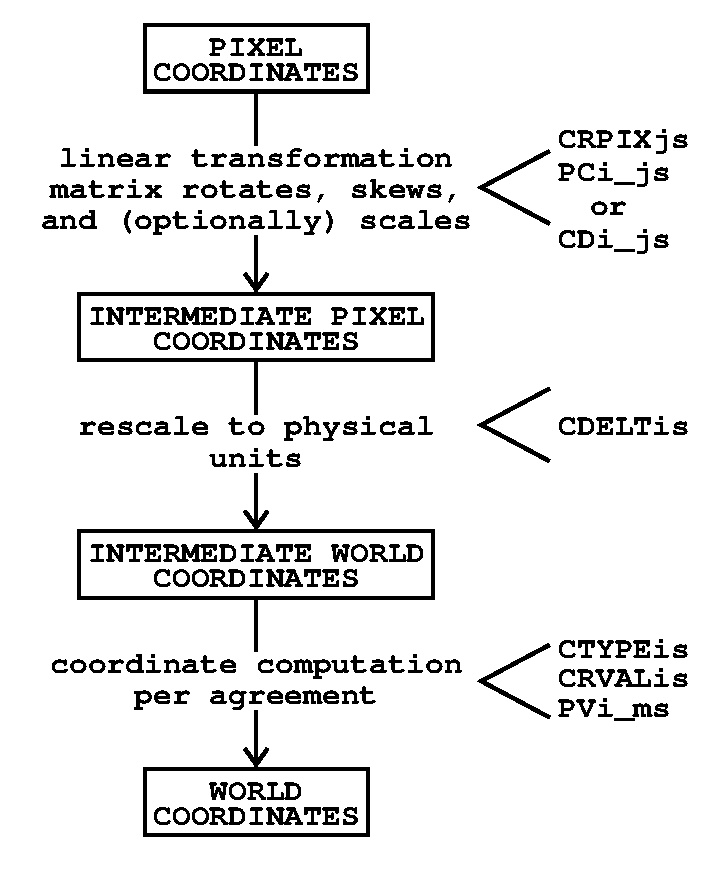
\includegraphics[width=.4\textwidth]{figures/process-wcs.eps}
  \qquad \qquad
  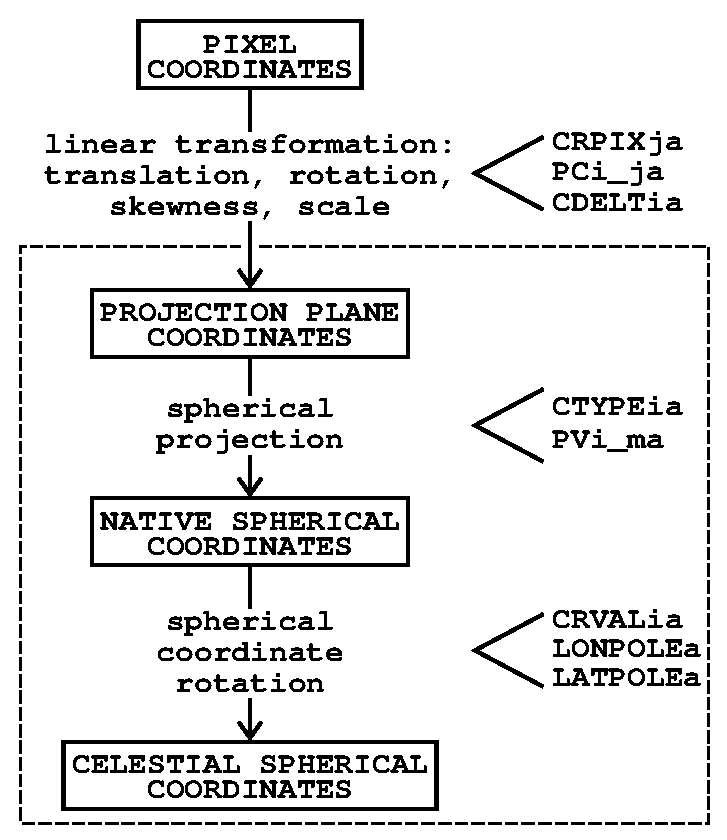
\includegraphics[width=.4\textwidth]{figures/process-ccs.eps}
  \caption[Conversion of pixel coordinates to world coordinates shown
    as a multi-step process]{Conversion of pixel coordinates to world coordinates shown
    as a multi-step process. (left)  In the first step a linear
    transformation is applied via matrix multiplication of the pixel
    coordinate vector.  This linear transformation may be restricted to
    the geometrical effects of rotation and skewness with scaling to
    physical units deferred until the second step (\PCij\ plus \CDELT{i}\
    formalism).  Alternatively, scaling may be applied via the matrix with
    the second step omitted (\CDij\ formalism).  The final step applies a
    possibly non-linear transformation to produce the final world
    coordinates.  Although generic keywords for this step are defined in
    this paper, the mathematical details, including the interpretation of
    the {\sc intermediate world coordinates}, are deferred to later papers
    which may also interpose additional steps in the algorithm chain. 
    (right) Conversion of pixel coordinates to celestial coordinates. The
    \textsc{intermediate world coordinates} of figure on the left are here
    interpreted as {\sc projection plane coordinates}, i.e.\ Cartesian
    coordinates in the plane of projection, and the multiple steps required to
    produce them have been condensed into one.}
  \label{fig:process-wcs}
\end{figure}

For all coordinate types, the first step is a linear transformation
applied via matrix multiplication to the vector of \textsl{pixel
  coordinate} elements, $p_{j}$:
\begin{eqnarray}
  \label{eq:6}
  q_{i} & = & \sum^{N}_{j=1} M_{ij} \left( p_{j} - r_{j} \right)
\end{eqnarray}
where $r_{j}$ are the pixel coordinate elements of the reference point
given by the \verb|REFERENCE_PIXEL|. Henceforth we will use $j$ for
pixel axis indexing and $i$ for the world axes. The $M_{ij}$ matrix is
a non-singular square matrix of dimensions $N \times N$.
The elements, $q_{i}$, of the resulting \textsl{intermediate pixel
  coordinate} vector are offsets, in dimenionless pixel units, from
the reference point along axes coincident with thosewith those of the
\textsl{intermediate world coordinates}. Thus the conversion of
$q_{i}$ to the corresponding intermediate world coordinate element,
$x_{i}$, is a simple scale:
\begin{eqnarray}
  \label{eq:7}
  x_i & = & s_i q_i
\end{eqnarray}
In the \texttt{PC} formalism, the matrix elements $M_{ij}$ are encoded
through the \texttt{PC} attribute and the $s_i$ as
\texttt{INCREMENT}. The default values for $M_{ij}$ are
\begin{eqnarray}
  \label{eq:8}
  M_{ij} & = & \left\{
    \begin{array}{lll}
      1.0 & & i = j \\
      0.0 & & i \neq j
    \end{array}
  \right.
\end{eqnarray}
The \texttt{PC} matrix must not be singular; it must have an inverse.

\subsection{Specification of units}

Unless agreed otherwise, units should conform with the recommendations of the
IAU Style Manual \cite{mcnally.1988}, though rather appearing in plain
character form \cite{george.1995, ochsenbein.1996} instead using the
notation typically used in a published paper. An overview of the
encoding of the basic units is shown on Tab.~\ref{tab:basic-units} below.

\begin{comment}
  Check definitions in table against table from \cite{pdg.rpp},
  p.~106.
\end{comment}

\begin{table}[ht]
  \centering
  \begin{tabular}{lll}
    \hline
    \textsc{Quantity} & \textsc{Unit string} & \textsc{Meaning} \\
    \hline \hline
    length               & \texttt{m}   & meter \\
    mass                 & \texttt{kg}  & kilogram \\
    time                 & \texttt{s}   & second \\
    plane angle          & \texttt{rad} & radian \\
    solid angle          & \texttt{sr}  & steradian \\
    temperature          & \texttt{K}   & kelvin \\
    electric current     & \texttt{A}   & ampere \\
    amount of substance  & \texttt{mol} & mole \\
    luminosity intensity & \texttt{cd}  & candela \\
    \hline
  \end{tabular}
  \caption{IAU-recommended basic units (table adopted from \cite{fits.paper3}).}
  \label{tab:basic-units}
\end{table}

\subsection{Separation between physical interpretation and storage mechanism}
\label{sec:abstraction-formalism}

Both from a technical and a conceptual point of it makes sense to
separate the physical interpretation of a coordinate from the
underlying storage mechanism (i.e. the container used to hold the
metadata). In order to illustrate the motivation for this type of
abstraction, consider coordinate information required for the various
types of data products as listed in Tab. \ref{tab:lofar_data_types} below:

\input coordinates_image_table

\begin{itemize}
\item \textsc{icd-003} (Beam-Formed Data) records stokes values as
  function of time and frequency
  \begin{eqnarray*}
    I & = & I (t,\nu)
  \end{eqnarray*}
  Due to the fact that the frequency values are spread across multiple
  frequency band, the coordinate axis is non-contiguous, thereby
  requiring storage of the frequencies in tabulated form; as a result
  of this the following combination or basic storage containers is employed:
\begin{lstlisting}
.
|- Linear
`- Tabular
\end{lstlisting}
However in order to allow easier interpretation of the coordinates in
terms of the encoded physical quantities, the following seems more favorable:
\begin{lstlisting}
.
|- Time
`- Spectral
\end{lstlisting}
  
\item \textsc{icd-004} (Radio Sky Image Cube) records data in the form
  \begin{eqnarray*}
    I & = & I (p,\nu,\mathrm{Dec},\mathrm{RA})
  \end{eqnarray*}
which translates into the following set of physical coordinates:
\begin{lstlisting}
.
|- Polarization          {Tabular}
|- Spectral              {Linear|Tabular}
`- Direction             {Direction}
\end{lstlisting}
Depending on the character of the spectral axis, the internal
representation can be done either using a linear or a tabular coordinate.

\item \textsc{icd-008} (Rotation Measure Synthesis Cube) records data
  in the form
  \begin{eqnarray*}
    I & = & I (p, \phi, \mathrm{Dec}, \mathrm{RA})
  \end{eqnarray*}
which translates into the following set of physical coordinates:
\begin{lstlisting}
.
|- Polarization
|- FaradayDepth
`- Direction
\end{lstlisting}
Depending on the distribution of the Faraday depth values, the
internal representation can be done either using a linear or a tabular coordinate:
\begin{lstlisting}
.                                 .
|- Polarization                   |- Polarization
|- Linear                         |- Tabular
`- Direction                      `- Direction
\end{lstlisting}

\item Consider the possible representations for the coordinates
  attached to a (total intensity) dynamic spectrum:
\begin{lstlisting}
.                  .                  .                    .
`- Linear [2]      |- Linear  [1]     |- Linear  [1]       |- Tabular [1]
                   `- Linear  [1]     `- Tabular [1]       `- Tabular [1]
\end{lstlisting}
  All of the above are valid representation, given how the values
  along the coordinate axes are distributed. On the other hand looking at
  this from the perspective of the physical quantities to be described,
\begin{lstlisting}
.
|- Time       [1]
`- Spectral   [1]
\end{lstlisting}
it becomes clear that separating the underlying storage structure from
the physical interpretation results in a much clearer and unified picture.
\end{itemize}

\section{Coordinates Group}
\label{sec:coordinates-group}

The Coordinates Group acts as a container to take up a collection of coordinates,
as described in the subsequent sections below. Besides this function as a
container -- grouping together embedded coordinate objects -- the
Coordinates Group also provides basic reference frame information,
which is required for the proper transformation of quantities to other
reference systems.

\begin{table}[ht]
 \centering
  \begin{tabular}{|lllp{5cm}|} 
    \hline
    \textsc{Field/Keyword} & \textsc{Type} & \textsc{Value} & \textsc{Description} \\
    \hline \hline
    \small{\verb|GROUPTYPE|} & \verb|string| & \verb|`Coordinates'| &
    Group type descriptor \\
    \small{\verb|REF_LOCATION_VALUE|}  & \verb|array<double,1>| &  &
    Numerical value(s) of the reference location \\
    \small{\verb|REF_LOCATION_UNIT|} & \verb|array<string,1>| &  &
    Physical unit(s) for the reference location \\
    \small{\verb|REF_LOCATION_FRAME|} & \texttt{string} &  &
    Identifier for the reference system of the location \\
    \small{\verb|REF_TIME_VALUE|} & \texttt{double} &  & Numerical value of the
    reference time \\
    \small{\verb|REF_TIME_UNIT|} & \texttt{string} &  & Physical unit of the
    reference time \\
    \small{\verb|REF_TIME_FRAME|} & \texttt{string} &  & Identifier for the reference
    time system used \\
    \small{\verb|NOF_COORDINATES|} & \texttt{int} & $N_{\rm Coord}$ & Number of
    embedded coordinate groups \\
    \small{\verb|NOF_AXES|} & \texttt{int} & $N_{\rm Axes} =
    \sum_{n}^{N_{\rm Coord}} N_{n,\rm Axes}$ & Cummulative number of
    coordinate axes, as from adding up the coordinate axes of the
    embedded coordinate objects/groups. \\
    \small{\verb|COORDINATE_TYPES|} & \verb|array<string,1>| &  &
    Coordinate types of the embedded coordinates. \\
    \hline
    \small{\verb|COORDINATE_{N}|} & \texttt{Group} &  & coordinate object
    container \\
    \hline
  \end{tabular}
  \caption{Components of a Coordinates group.}
  \label{tab:coordinates-group} 
\end{table}

\begin{lstlisting}
.
`- COORDINATES                Group     
   |- GROUPTYPE               Attr.     string
   |- REF_LOCATION_VALUE      Attr.     array<double,1>
   |- REF_LOCATION_UNIT       Attr.     array<string,1>
   |- REF_LOCATION_FRAME      Attr.     array<string,1>
   |- REF_TIME_VALUE          Attr.     double
   |- REF_TIME_UNIT           Attr.     string
   |- REF_TIME_FRAME          Attr.     string
   |- NOF_COORDINATES         Attr.     int
   |- NOF_AXES                Attr.     int
   |- COORDINATE_TYPES        Attr.     array<string,1>
   |- COORDINATE_0            Group
   |   ...
   `- COORDINATE_{N}          Group
\end{lstlisting}

\begin{comment}
  Do we need description of the quantity to which the coordinates are
  attached to (see e.g. FITS keywords `BUNIT' and `BSCALE')?
\end{comment}

\begin{list}{\textbf{--}}{}
\item \verb|GROUPTYPE| is the group type descriptor with the fixed value
  \verb|`Coordinates'|.
\item Specification of the reference frame/system within which the
  location is recorded is done through the combination of \verb|REF_LOCATION_VALUE|,
  \verb|REF_LOCATION_UNIT| and \verb|REF_LOCATION_FRAME|; recognized
  values for the specification of the reference frame are listed in
  Tab. \ref{tab:reference-frames-location} below.
  
  \begin{table}[ht]
    \centering
    \begin{tabular}{|p{3.5cm}p{6cm}p{5cm}|}
      \hline
      \textsc{Reference~Position} & \textsc{Description} & \textsc{Comments} \\
      \hline \hline
      \verb|GEOCENTER|    & Center of the Earth. & \\
      \verb|BARYCENTER|   & Center of the solar system barycenter. &  \\
      \verb|HELIOCENTER|  & Center of the Sun. &  \\
      \verb|TOPOCENTER|   & ``Local''; in most cases this will mean:
      the location of the telescope. &  \\
      \verb|LSRK|         & Kinematic Local Standard of Rest: 20 km
      s$^{-1}$ in the direction of \verb|GALACTIC_II| $(56,+23)$. & Only to be
      used for redshifts and Doppler velocities, and spectral coordinate. \\
      \verb|LSRD|         & Dynamic Local Standard of Rest: 16.6 km
      s$^{-1}$ in the direction of \verb|GALACTIC_II| $(53,+25)$. &  \\
      \verb|GALACTIC|     & Center of the Galaxy: 220 km s$^{-1}$ in
      the direction of \verb|GALACTIC_II| $(90,0)$ w.r.t. \texttt{LSRD}. &  \\
      \verb|LOCAL_GROUP|  & Center of the Local Group: 300 km s$^{-1}$ in
      the direction of \verb|GALACTIC_II| $(90,0)$ w.r.t. \texttt{BARYCENTER}. &  \\
      \verb|RELOCATABLE|  & Relocatable center; for simulations. & Only to be used
      for spatial coordinates. \\
      \hline
    \end{tabular}
    \caption[Recognized values for the reference frame to specify a
      location]{Recognized values for the reference frame to specify a
      location; values and descriptions have been adopted from the
      ``Space-Time Coordinate Metadata for the Virtual Observatory''
      \cite{ivoa.stc}, as produced by the IVOA Data Model Working Group.}
    \label{tab:reference frames location}
  \end{table}
  
\item Specification of the reference frame/system within which the
  time/epoch is recorded is done through the combination of
  \verb|REF_TIME_VALUE|, \verb|REF_TIME_UNIT| and
  \verb|REF_TIME_FRAME|; recognized values for the specification of
  the reference frame are listed in Tab. \ref{tab:reference-frames-time} below.
  
  \begin{table}[ht]
    \centering
    \begin{tabular}{|p{3cm}p{11cm}|}
      \hline
      \textsc{Time} & \textsc{Description} \\
      \hline \hline
      \texttt{GAST} & Greenwich Apparent Sidereal Time \\
      \texttt{GMST} & Greenwich Mean Sidereal Time \\
      \texttt{LAST} & Local Apparent Sidereal Time \\
      \texttt{LMST} & Local Mean Sidereal Time \\
      \texttt{TAI}  & International Atomic Time \\
      \texttt{TCB}  & Barycentric Coordinate Time \\
      \texttt{TCG}  & Geocentric Coordinate Time \\
      \texttt{TDB}  & Barycentric Dynamical Time \\
      \texttt{TT}   & Terrestrial Time \\
      \texttt{UT1}  & Universal Time (affected by variations in length
      of day) \\
      \texttt{UTC}  & Coordinated Universal Time (an atomic tim scale) \\
      \hline
    \end{tabular}
    \caption{Recognized values for the reference frame to specify a
      time; descriptions adopted from \cite{kaplan.2000}}
    \label{tab:reference-frames-time}
  \end{table}
  
  For the SI-based time scales, the event tagged 1977 January 1,
  00:00:00 TAI (JD 2443144.5 TAI) at the geocenter is special. At that
  event, the time scales TT, TCG, and TCB all read 1977 January 1,
  00:00:32.184 (JD 2443144.5003725). (The 32$^s$.184 offset is the
  estimated difference between TAI and the old Ephemeris Time scale.)
  This event will be designated $t_0$ in the following; it can be
  represented in any of the time scales, and the context will dictate
  which time scale is appropriate. 

  \begin{comment}
    Get reference for definition of time reference frames.
  \end{comment}

  From the perspective of a user, the starting point for computing all
  the time scales is Coordinated Universal Time (UTC). From UTC, we
  can immediately get International Atomic Time (TAI):
  \begin{eqnarray*}
    \mathrm{TAI} & = & \mathrm{UTC} + \Delta \mathrm{AT}
  \end{eqnarray*}
  where $\Delta$AT, an integral number of seconds, is the accumulated
  number of leap seconds applied to UTC.
\item Since the coordinates group acts as a container for multiple
  coordinate (objects), \verb|NOF_COORDINATES| accounts for the number
  of such coordinates.
\item Since a coordinate can be composed of multiple axes (e.g. a
  Direction Coordinate consists of two direction angles),
  \verb|NOF_AXES| accounts for the total number of cordinates axes.
\item \verb|COORDINATE_TYPES|
\end{list}

%%_______________________________________________________________________________
%%                                           Subsection: Basic storage containers

\section{Basic storage containers}
\label{sec:storage-containers}

%%_______________________________________________________________________________
%%                                                           Direction coordinate

\subsection{Direction coordinate}
\label{sec:coord-direction}

The Direction Coordinate consists of a set of two coupled coordinate
axes, describing a direction in space; it therefore includes
information such as the equinox of the observation, the system of
equatorial coordinates on the sphere of the sky, as well as parameters
for the spherical map projection.

\input coordinates_coord_direction_table

\begin{lstlisting}[float,caption={Structure of the direction
    coordinate group.}]
.
`- COORDINATE_{N}           Group
   |- GROUPTYPE             Attr.       string
   |- COORDINATE_TYPE       Attr.       string
   |- STORAGE_TYPE          Attr.       string
   |- NOF_AXES              Attr.       int
   |- AXIS_NAMES            Attr.       array<string,1>
   |- AXIS_UNITS            Attr.       array<string,1>
   |- REFERENCE_VALUE       Attr.       array<double,1>
   |- REFERENCE_PIXEL       Attr.       array<double,1>
   |- INCREMENT             Attr.       array<double,1>
   |- PC                    Attr.       array<double,1>
   |- EQUINOX               Attr.       string
   |- RADEC_SYS             Attr.       string
   |- PROJECTION            Attr.       string
   |- PROJECTION_PARAM      Attr.       array<double,1>
   |- LONGPOLE              Attr.       double
   `- LATPOLE               Attr.       double
\end{lstlisting}

\begin{list}{\textbf{--}}{}
\item \verb|GROUPTYPE| is the group type descriptor with the fixed value
  \verb|`DirectionCoord'|.
\item \verb|COORDINATE_TYPE| is the is the descriptor for the
  coordinate type, of value \verb|`Direction'|.
\item \verb|STORAGE_TYPE| is the descriptor for the underlying storage
  type for this coordinate, of value \verb|`Direction'|.
\item \verb|NOF_AXES| is the number of coordinate axes; keep in mind
  that a coordinate can consist of multiple axes. For the the
  DirectionCoordinate we have \verb|NOF_AXES=2|.
\item \verb|AXIS_NAMES| are the world axis names connected with the
  coordinate axes,most commonly
  \begin{verse}
    \verb|AXIS_NAME=[`Longitude',`Latitude']|
  \end{verse}
\item \verb|AXIS_UNITS| are the physical units along each coordinate axis
  (corresponding to the FITS keyword \verb|CUNITn|, see \cite{fits.paper1}).
  Restrictions on the nature and range of units, if any, will be determined by
  agreements applying to the specific axis. If they are not so limited, units
  should conform to the IAU Style Manual \cite{mcnally.1988}.
\item \verb|REFERENCE_VALUE| is the coordinate value at the reference point
   (corresponding to the FITS keyword \CRVAL{n}, see \cite{fits.paper1}).
\item \verb|REFERENCE_PIXEL| is the array location of the reference point in 
  pixels (corresponding to the FITS keyword \CRPIX{n}, see \cite{fits.paper1}).
\item \verb|INCREMENT| is the coordinate increment at the reference point
   (corresponding to the FITS keyword \CDELT{n}, see \cite{fits.paper1}).
\item \verb|PC| is a non-singular square matrix, for the
  transformation from intermediate pixel coordinates to intermediate
  world coordinates. The individual matrix elements are stored as a
  linear array, ordered as follows:
  \begin{eqnarray*}
     \mathbf{M}_{[N,N]} \ = \ \left(
       \begin{array}{cccc}
         M_{00}  & M_{01} & ... & M_{0N} \\
         M_{10}  & M_{11} & ... & M_{1N} \\
         \vdots  &       &     & \vdots \\
         M_{N0}  &        &     & M_{NN}
       \end{array}
     \right) 
     & \rightarrow &
     \left[ M_{00}, M_{01}, ... , M_{10}, M_{11}, ..., M_{N0}, ..., M_{NN} \right]
  \end{eqnarray*}
\item \verb|EQUINOX| applies to ecliptic as well as to equatorial
  coordinates (e.g. \texttt{J2000} or \texttt{B1950}) of the source position.
\item \verb|RADEC_SYS| Several systems of equatorial coordinates
  (right ascension and declination) are in common use. Apart from the
International Celestial Reference System (ICRS, IAU, 1984), the axes
of which are by definition fixed with respect to the celestial sphere, each
  system is parameterized by time. In particular, mean equatorial
  coordinates are defined in terms of the epoch (i.e.\ instant of
  time) of the mean equator and equinox (i.e.\ pole and origin of
  right ascension). The same applies for ecliptic coordinate
  systems. The keyword \verb|RADEC_SYS| is used to specify the
  particular system; recognized values are given in
  Tab. \ref{tab:radec-sys} below.
  \begin{table}[ht]
    \centering
    \begin{tabular}{ll}
      \hline
      \verb|RADEC_SYS| & \textsc{Description} \\
      \hline \hline
      \verb|ICRS|     & International Celestial Reference System \\
      \verb|FK5|      & mean place, new (IAU 1984) system \\
      \verb|FK4|      & mean place, old (Bessell-Newcomb) system \\
      \verb|FK4-NO-E| & meanplace, old system but without e-terms \\
      \verb|GAPPT|    & Geocentric Apparent Place, IAU 1984 system \\
      \hline
    \end{tabular}
    \caption{Allowed values of \texttt{RADEC$_-$SYS}}
    \label{tab:radec-sys}
  \end{table}
\item \verb|PROJECTION| holds the reference code for the spherical map
  projection, e.g. \texttt{AIT}, \texttt{SIN}, \texttt{STG},
  etc. As some of these projections require (or at least allow)
  additional parameters, the \verb|PROJECTION_PARAM| keyword is used
  to store these additional parameters. Recognized values are given in
  Table \ref{tab:projections} below.
  \begin{table}[ht]
    \centering
    \begin{tabular}{llcll}
      \hline
      \multicolumn{2}{c}{\sc Projection} &
      $\phi_0$ &
      $\theta_0$ &
      \textsc{Projection parameters}\\
      \hline \hline
      \keyv{AZP} & Zenithal perspective
      & $0^\circ$ & $90^\circ$
      & $[ \mu, \gamma ]$ \\
      \keyv{SZP} & Slant zenithal perspective
      & $0^\circ$ & $90^\circ$
      & $[ \mu, \phi_{c}, \theta_{c} ]$ \\
      \keyv{TAN} & Gnomonic
      & $0^\circ$ & $90^\circ$
      \\
      \keyv{STG} & Stereographic
      & $0^\circ$ & $90^\circ$
      \\
      \keyv{SIN} & Slant orthographic
      & $0^\circ$
      & $90^\circ$
      & $[ \xi, \eta ]$ \\
      \keyv{ARC} & Zenithal equidistant
      & $0^\circ$
      & $90^\circ$
      \\
      \keyv{ZPN} & Zenithal polynomial
      & $0^\circ$
      & $90^\circ$
      & $[ P_0, P_1, .. , P_m ]$ for $m = 0,\ldots 29$ \\
      \keyv{ZEA} & Zenithal equal-area
      & $0^\circ$
      & $90^\circ$
      \\
      \keyv{AIR} & Airy
      & $0^\circ$
      & $90^\circ$
      & $[ \theta_{b}] $
      \\
      \noalign{\medskip}
      \keyv{CYP} & Cylindrical perspective
      & $0^\circ$
      & $0^\circ$
      & $[ \mu, \lambda ]$
      \\
      \keyv{CEA}
      & Cylindrical equal area
      & $0^\circ$
      & $0^\circ$
      & $[ \lambda ]$
      \\
      \keyv{CAR}
      & Plate carr\'{e}e
      & $0^\circ$
      & $0^\circ$
      \\
      \keyv{MER}
      & Mercator
      & $0^\circ$
      & $0^\circ$
      \\
      \noalign{\medskip}
      \keyv{SFL}
      & Sanson-Flamsteed
      & $0^\circ$
      & $0^\circ$
      \\
      \keyv{PAR}
      & Parabolic
      & $0^\circ$
      & $0^\circ$
      \\
      \keyv{MOL}
      & Mollweide
      & $0^\circ$
      & $0^\circ$
      \\
      \keyv{AIT} & Hammer-Aitoff
      & $0^\circ$
      & $0^\circ$
      \\
      \noalign{\medskip}
      \keyv{COP} & Conic perspective
      & $0^\circ$
      & $\theta_{a}$
      & $[ \theta_{a}, \eta] $
      \\
      \keyv{COE} & Conic equal-area
      & $0^\circ$
      & $\theta_{a}$
      & $[ \theta_{a}, \eta] $
      \\
      \keyv{COD} & Conic equidistant
      & $0^\circ$
      & $\theta_{a}$
      & $[ \theta_{a}, \eta] $
      \\
      \keyv{COO} & Conic orthomorphic
      & $0^\circ$
      & $\theta_{a}$
      & $[ \theta_{a}, \eta] $
      \\
      \noalign{\medskip}
      \keyv{BON}
      & Bonne's equal area
      & $0^\circ$
      & $0^\circ$
      & $[ \theta_1 ]$ \\
      \keyv{PCO}
      & Polyconic
      & $0^\circ$
      & $0^\circ$
      \\
      \noalign{\medskip}
      \keyv{TSC}
      & Tangential Spherical Cube
      & $0^\circ$
      & $0^\circ$
      \\
      \keyv{CSC}
      & COBE Quadrilateralized Spherical Cube
      & $0^\circ$
      & $0^\circ$
      \\
      \keyv{QSC}
      & Quadrilateralized Spherical Cube
      & $0^\circ$
      & $0^\circ$
      \\
      \noalign{\smallskip}
      \hline
    \end{tabular}
    \caption[Summary of projection codes]{Summary of projection codes, full name, default values of $\phi_0$ and
      $\theta_0$, and required parameters. Values and descriptions have
      been adopted from \cite{fits.paper2}.}
    \label{tab:projections}
  \end{table}
  \begin{figure}[ht]
    \centering
    \includegraphics[width=.3\textwidth]{figures/projection-tan.eps}
    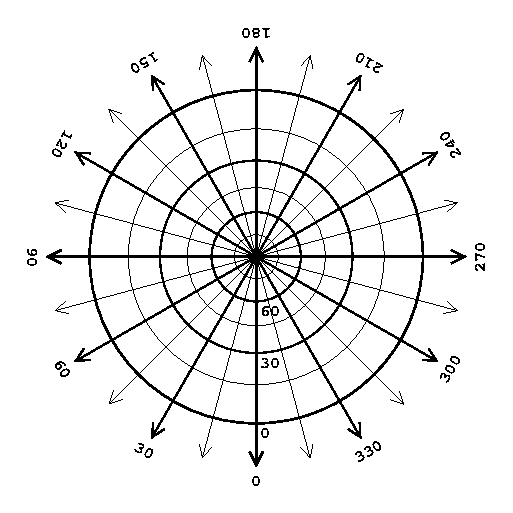
\includegraphics[width=.3\textwidth]{figures/projection-stg.eps}
    \includegraphics[width=.3\textwidth]{figures/projection-zea.eps} \\
    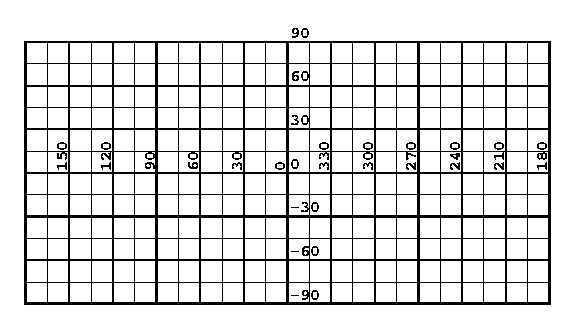
\includegraphics[width=.45\textwidth]{figures/projection-car.eps}
    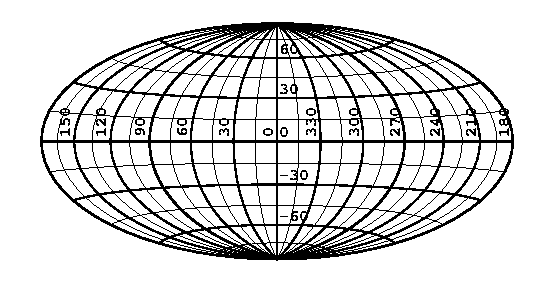
\includegraphics[width=.45\textwidth]{figures/projection-ait.eps}
    \caption[A selection of spherical map projections]{A selection of spherical map projections. Top row, from
      left to right: \keyv{TAN} (Gnomonic), \keyv{STG} (Stereographic),
      \keyv{ZEA} (Zenithal equal-area). Bottom row, from left to right:
      \keyv{CAR} (Plate carr\'{e}e), \keyv{AIT} (Hammer-Aitoff).}
    \label{fig:projections}
  \end{figure}
\item \verb|LONPOLE| is the native longitude of the celestial pole, $\phi_p$.
\item \verb|LATPOLE| is the native latitude of the celestial pole, $\theta_p$.
\end{list}

%%_______________________________________________________________________________
%%                                                              Linear coordinate

\subsection{Linear coordinate}
\label{sec:coord-linear}

As already indicated by the name, this group encodes the properties of a simple
linear coordinate (or a number thereof, as multiple axes are permitted).

\input coordinates_coord_linear_table

\begin{lstlisting}[float,caption={Structure of the linear coordinate group.}]
.
`- COORDINATE_{N}           Group
   |- GROUPTYPE             Attr.       string
   |- COORDINATE_TYPE       Attr.       string
   |- STORAGE_TYPE          Attr.       string
   |- NOF_AXES              Attr.       int
   |- AXIS_NAMES            Attr.       array<string,1>
   |- AXIS_UNITS            Attr.       array<string,1>
   |- REFERENCE_VALUE       Attr.       array<double,1>
   |- REFERENCE_PIXEL       Attr.       array<double,1>
   |- INCREMENT             Attr.       array<double,1>
   `- PC                    Attr.       array<double,1>
\end{lstlisting}

\begin{list}{\textbf{--}}{}
\item \verb|GROUPTYPE| is the group type descriptor with the fixed value
  \verb|`LinearCoord'|. 
\item \verb|COORDINATE_TYPE| is the is the descriptor for the
  coordinate type, of value \verb|`Linear'|.
\item \verb|STORAGE_TYPE| is the descriptor for the underlying storage
  type for this coordinate, of value \verb|`Linear'|.
\item \verb|NOF_AXES| is the number of coordinate axes represented by
  this coordinate.
\item \verb|AXIS_NAMES| are the world axis names connected with the
  coordinate axes, e.g.
  \begin{verse}
    \verb|AXIS_NAMES=[`Distance']| \\
    \verb|AXIS_NAMES=[`Time']| \\
    \verb|AXIS_NAMES=[`Azimuth',`Elevation']|
  \end{verse}
\item \verb|AXIS_UNITS| are the physical units along each coordinate axis
  (corresponding to the FITS keyword \verb|CUNITi|, see \cite{fits.paper1}).
  Restrictions on the nature and range of units, if any, will be determined by
  agreements applying to the specific axis. If they are not so limited, units
  should conform to the IAU Style Manual \cite{mcnally.1988}.
\item \verb|REFERENCE_VALUE| is the coordinate value at the reference point
   (corresponding to the FITS keyword \CRVAL{n}, see \cite{fits.paper1}).
\item \verb|REFERENCE_PIXEL| is the array location of the reference point in 
  pixels (corresponding to the FITS keyword \CRPIX{n}, see \cite{fits.paper1}).
\item \verb|INCREMENT| is the coordinate increment at the reference point
   (corresponding to the FITS keyword \CDELT{n}, see \cite{fits.paper1}).
\item \verb|PC| is a non-singular square matrix, for the
  transformation from intermediate pixel coordinates to intermediate
  world coordinates. The individual matrix elements are stored as a
  linear array, ordered as follows:
  \begin{eqnarray*}
     \mathbf{M}_{[N,N]} \ = \ \left(
       \begin{array}{cccc}
         M_{00}  & M_{01} & ... & M_{0N} \\
         M_{10}  & M_{11} & ... & M_{1N} \\
         \vdots  &       &     & \vdots \\
         M_{N0}  &        &     & M_{NN}
       \end{array}
     \right) 
     & \rightarrow &
     \left[ M_{00}, M_{01}, ... , M_{10}, M_{11}, ..., M_{N0}, ..., M_{NN} \right]
  \end{eqnarray*}
\end{list}


\subsection{Tabular coordinate}
\label{sec:coord-tabular}

\input coordinates_coord_tabular_table

\begin{lstlisting}[float,caption={Structure of the tabular coordinate group.}]
.
`- COORDINATE_{N}
   |- GROUPTYPE             Group       string
   |- COORDINATE_TYPE       Attr.       string
   |- STORAGE_TYPE          Attr.       string
   |- NOF_AXES              Attr.       int
   |- AXIS_NAMES            Attr.       array<string,1>
   |- AXIS_UNITS            Attr.       array<string,1>
   |- AXIS_LENGTH           Attr.       int
   |- AXIS_VALUES_PIXEL     Attr.       array<double,1>
   `- AXIS_VALUES_WORLD     Attr.       array<double,1>
\end{lstlisting}

\begin{list}{\textbf{--}}{}
\item \verb|GROUPTYPE| is the group type descriptor with the fixed value 
  \verb|`TabularCoord'|. 
\item \verb|COORDINATE_TYPE| is the is the descriptor for the
  coordinate type, of value \verb|`Tabular'|.
\item \verb|STORAGE_TYPE| is the descriptor for the underlying storage
  type for this coordinate, of value \verb|`Tabular'|.
\item \verb|NOF_AXES| is the number of coordinate axes; keep in mind that a
  coordinate can consist of multiple axes.
\item \verb|AXIS_NAMES| are the world axis names connected with the
  coordinate axes, e.g.
  \begin{verse}
    \verb|AXIS_NAME=[`Distance']| \\
    \verb|AXIS_NAME=[`Time']|
  \end{verse}
\item \verb|AXIS_UNITS| are the physical units along each coordinate axis
  (corresponding to the FITS keyword \verb|CUNITi|, see \cite{fits.paper1}).
  Restrictions on the nature and range of units, if any, will be determined by
  agreements applying to the specific axis. If they are not so limited, units
  should conform to the IAU Style Manual \cite{mcnally.1988}.
\item \verb|AXIS_VALUES_PIXEL| are the tabulated values of pixel coordinates.
\item \verb|AXIS_VALUES_WORLD| are the tabulated values of world coordinates.
\end{list}

\subsection{Composite containers}
\label{sec:composite-containers}

\subsection{Time coordinate}
\label{sec:coord-time}

Given the characteristics of the time axis, a time coordinate internal
will either be storing its values as a linear axis
(\verb|STORAGE_TYPE=`Linear'|) or as a 1-dimensional look-up table
(\verb|STORAGE_TYPE=`Tabular'|).

\input coordinates_coord_time_table

\begin{list}{\textbf{--}}{}
\item \verb|GROUPTYPE| is the group type descriptor with the fixed
  value \verb|`TimeCoord'|.
\item \verb|COORDINATE_TYPE| is the coordinate type descriptor with
  the fixed value \verb|`Time'|.
\item \verb|STORAGE_TYPE| indicates the underlying storage mechanism: if 
  \verb|STORAGE_TYPE=`Linear'| the coordinate axis is expected to be linear and
  represented by the attributes defined for a Linear Coordinate (see section
  \ref{sec:coord-linear}). If set \verb|STORAGE_TYPE=`Tabular'|, the values along
  the coordinate axis are expected to be tabulated, thereby represented by the
  attributes defined for a Tabular Coordinate (see section
  \ref{sec:coord-tabular}).
  \begin{comment}
    Add description of structure depending on storage type.
  \end{comment}
\item \verb|REFERENCE_FRAME| records the reference frame within which
  the time coordinate axis is defined; see
  Tab.~\ref{tab:reference-frames-time} for a list of recognized
  values. This can be a diferent frame as used for e.g. the direction
  coordinate or as noted in the coordinates group. 
\item \verb|NOF_AXES| is the number of coordinate axes.
\item \verb|AXIS_NAMES| are the world axis names connected with the
  coordinate axes, i.e. \verb|AXIS_NAMES=[`Time']|.
\item \verb|AXIS_UNITS| are the physical units world axis of the coordinate
  (corresponding to the FITS keyword \verb|CUNITi|, see \cite{fits.paper1}).
  Restrictions on the nature and range of units, if any, will be determined by
  agreements applying to the specific axis. If they are not so limited, units
  should conform to the IAU Style Manual \cite{mcnally.1988}.
\end{list}

%%_______________________________________________________________________________
%%                                                            Spectral coordinate

\subsection{Spectral coordinate}
\label{sec:coord-spectral}

Spectral coordinates are commonly given in units of frequency,
wavelength, velocity, and other parameters proportional to these
three \cite{fits.paper3}. The coordinate types discussed here are then frequency,
wavelength, and “apparent radial velocity” denoted by the symbols
$\nu$, $\lambda$, and $v$. There are also three conventional
velocities frequently used in astronomy. These are the so-called
“radio” velocity, “optical” velocity, and redshift, denoted here by
$V$, $Z$, and $z$ and given by
\begin{displaymath}
  V \ = \ c \ \frac{\nu_{0} - \nu}{\nu_{0}} \ , \qquad
  Z \ = \ c \ \frac{\lambda-\lambda_0}{\lambda_0} \quad \hbox{and} \qquad
  z \ = \ Z/c \ .
\end{displaymath}
The velocities are defined so that an object receding from the observer has a
positive velocity. Table \ref{tab:spectral coordinate codes} below
lists the various spectral quantities and their respective encoding as
an attribute; the symbols $\lambda_{0}$ and $\nu_{0}$ are the rest
wavelength and frequency, respectively, of the spectral line used to
associate velocity with observed wavelength and frequency.

\begin{table}[htb]
  \centering
  \begin{tabular}{lp{1.5cm}llp{1.5cm}p{1.5cm}}
    \hline
    \textsc{Attribute} & \textsc{FITS Code} & \textsc{Name} &
    \textsc{Symbol} & Associate variable & Default units \\
    \hline \hline
    \verb|Frequency|       & \verb|FREQ| & Frequency  & $\nu$ & $\nu$ & Hz \\
    \verb|Energy|          & \verb|ENER| & Energy     & $E$   & $\nu$ & J  \\
    \verb|Wavenumber|      & \verb|WAVN| & Wavenumber & $\kappa$ & $\nu$ & m$^{-1}$ \\
    \verb|VelocityRadio|   & \verb|VRAD| & Radio velocity & $V$ & $\nu$ & m s$^{-1}$ \\
    \verb|VelocityOptical| & \verb|VOPT| & Optical velocity & $Z$ & $\lambda$ & m s$^{-1}$ \\
    \verb|VelocityAppRadial| & \verb|VELO| & Apparent radial velocity & $v$ & $v$ & m s$^{-1}$ \\
    \verb|Redshift|        & \verb|ZOPT| & Redshift    & $z$ & $\lambda$ & -- \\
    \verb|WavelengthVacuum|& \verb|FREQ| & Vacuum wavelength & $\lambda$ & $\lambda$ & m \\
    \verb|WavelengthAir|   & \verb|AWAV| & Air wavelength  & $\lambda_a$ & $\lambda_a$ & m \\
    \verb|BetaFactor|      & \verb|BETA| & Beta factor $v/c$  & $\beta$ & $v$ & -- \\
    \hline
  \end{tabular}
  \caption[Attributes values corresponding to the spectral coordinate
    codes]{Attributes values corresponding to the spectral coordinate
    codes, as defined in \cite{fits.paper3}. The IAU-standard prefixes
    for scaling the unit are described in \cite{fits.paper1} and
    should be used with al coordinate types, except that the
    dimensionless ones are not scaled.}
  \label{tab:spectral coordinate codes}
\end{table}

\begin{table}[htbp]
  \centering
  \begin{tabular}{lll}
    \hline
    \textsc{Name} & \textsc{Symbol} & \textsc{Transformation equation(s)} \\
    \hline \hline
    \\[-1mm]
    Frequency & $\nu$ & $\displaystyle \nu \ = \ c/\lambda \ = \ E/h$ \\[3mm]
    Vacuum wavelength & $\lambda$ & $\displaystyle \lambda\ = \ c/\nu \ =
    \ \lambda_{0} \ \frac{c+v}{\sqrt{c^2 - v^2}}$ \\[3mm]
    Apparent radial velocity & $v$ & $\displaystyle v \ = \ c \ 
    \frac{\nu_{0}^{2} - \nu^{2}}{\nu_{0}^{2} + \nu^{2}} \ = \ c \ 
    \frac{\lambda^{2} - \lambda_{0}^{2}}{\lambda^{2} +
      \lambda_{0}^{2}} $ \\[4mm]
    \hbox{Energy} & $E$ & $\displaystyle E = h \nu$ \\[3mm]
    \hbox{Redshift} & $z$ & $\displaystyle z \ = \
    \frac{\lambda-\lambda_{0}}{\lambda}$ \\[2mm]
    \hline
  \end{tabular}
  \caption[Spectral transformation equations]{Spectral transformation equations; for the full set
    of equations -- including first order derivatives -- see \cite{fits.paper3}.}
  \label{tab:spectral transformations}
\end{table}

As it turns out, providing a set of parameters to properly describe a spectral
coordinate is not straight-forward: given the arrangement of frequency channels
or bands the values along the coordinate axis might be linear, but
does not necessarily have to be. Therefore in principle a spectral
coordinate can be considered a derivative of either a linear or a
tabular coordinate, with a number of specific attributes added, as
they will be required for the transformation between different
spectral quantities.

\input coordinates_coord_spectral_table

\begin{list}{\textbf{--}}{}
\item \verb|GROUPTYPE| is the group type descriptor with the fixed value \verb|`SpectralCoord'|.
\item \verb|COORDINATE_TYPE| is the coordinate type descriptor with the fixed value
  `SPECTRAL'.
\item \verb|NOF_AXES| is the number of coordinate axes.
\item \verb|AXIS_NAMES| are the world axis names associated with the
  spectral coordinates, e.g.
  \begin{verse}
    \verb|AXIS_NAMES=[`Frequency']| \\
    \verb|AXIS_NAMES=[`WavelengthVacuum']|
  \end{verse}
  Allowed and supported values are listed in Tab.~\ref{tab:spectral
    coordinate codes} above.
\item \verb|AXIS_UNITS| are the physical units along each coordinate axis
  (corresponding to the FITS keyword \verb|CUNITi|, see \cite{fits.paper1}).
  Restrictions on the nature and range of units, if any, will be determined by
  agreements applying to the specific axis. If they are not so limited, units
  should conform to the IAU Style Manual \cite{mcnally.1988}.
\item \verb|STORAGE_TYPE| indicates the underlying storage mechanism: if 
  \verb|STORAGE_TYPE=`Linear'| the coordinate axis is expected to be linear and
  represented by the attributes defined for a Linear Coordinate:
  \begin{lstlisting}
.
`- COORDINATE_{N}           Group
   |- GROUPTYPE             Attr.       string
   |- COORDINATE_TYPE       Attr.       string
   |- STORAGE_TYPE          Attr.       string
   |- REFERENCE_FRAME       Attr.       string
   |- REST_FREQUENCY        Attr.       double
   |- REST_FREQUENCY_UNIT   Attr.       string
   |- REST_WAVELENGTH       Attr.       double
   |- REST_WAVELENGTH_UNIT  Attr.       string
   |- NOF_AXES              Attr.       int
   |- AXIS_NAMES            Attr.       array<string,1>
   |- AXIS_UNITS            Attr.       array<string,1>
   |- REFERENCE_VALUE       Attr.       array<double,1>
   |- REFERENCE_PIXEL       Attr.       array<double,1>
   |- INCREMENT             Attr.       array<double,1>
   `- PC                    Attr.       array<double,1>
 \end{lstlisting}
 In this:
 \begin{itemize}
 \item \verb|REFERENCE_VALUE| is the coordinate value at the reference point
   (corresponding to the FITS keyword \CRVAL{n}, see \cite{fits.paper1}).
 \item \verb|REFERENCE_PIXEL| is the array location of the reference point in 
   pixels (corresponding to the FITS keyword \CRPIX{n}, see \cite{fits.paper1}).
 \item \verb|INCREMENT| is the coordinate increment at the reference point
   (corresponding to the FITS keyword \CDELT{n}, see \cite{fits.paper1}).
 \item \verb|PC| is a non-singular square matrix, for the
   transformation from intermediate pixel coordinates to intermediate
   world coordinates. The individual matrix elements are stored as a
   linear array, ordered as follows:
   \begin{eqnarray*}
     \mathbf{M}_{[N,N]} \ = \ \left(
       \begin{array}{cccc}
         M_{00}  & M_{01} & ... & M_{0N} \\
         M_{10}  & M_{11} & ... & M_{1N} \\
         \vdots  &       &     & \vdots \\
         M_{N0}  &        &     & M_{NN}
       \end{array}
     \right) 
     & \rightarrow &
     \left[ M_{00}, M_{01}, ... , M_{10}, M_{11}, ..., M_{N0}, ..., M_{NN} \right]
   \end{eqnarray*}
 \end{itemize}
 If set \verb|STORAGE_TYPE=`Tabular'|, the values along
 the coordinate axis are expected to be tabulated, thereby represented by the
 attributes defined for a Tabular Coordinate:
 \begin{lstlisting}
.
`- COORDINATE_{N}           Group
   |- GROUPTYPE             Attr.       string
   |- COORDINATE_TYPE       Attr.       string
   |- STORAGE_TYPE          Attr.       string
   |- REFERENCE_FRAME       Attr.       string
   |- REST_FREQUENCY        Attr.       double
   |- REST_FREQUENCY_UNIT   Attr.       string
   |- REST_WAVELENGTH       Attr.       double
   |- REST_WAVELENGTH_UNIT  Attr.       string
   |- NOF_AXES              Attr.       int
   |- AXIS_NAMES            Attr.       array<string,1>
   |- AXIS_UNITS            Attr.       array<string,1>
   |- AXIS_LENGTH           Attr.       int
   |- AXIS_VALUES_PIXEL     Attr.       array<double,1>
   `- AXIS_VALUES_WORLD     Attr.       array<double,1>
 \end{lstlisting}
 In this:
 \begin{itemize}
 \item \verb|AXIS_LENGTH| is the length of the tabulated axis,
   i.e. the number of elements stored in the \verb|AXIS_VALUES_PIXEL|
   and \verb|AXIS_VALUES_WORLD| arrays.
 \item \verb|AXIS_VALUES_PIXEL| are the tabulated values along the pixel
    axis.
 \item \verb|AXIS_VALUES_WORLD| are the tabulated values along the world
    axis.
 \end{itemize}
\end{list}

%% ______________________________________________________________________________
%%                                                        Polarization coordinate

\subsection{Polarization coordinate}
\label{sec:coord-polarization}

\paragraph{Definition of physical parameters.}

The Stokes parameters are a set of values that describe the
polarization state of electromagnetic radiation. They were defined as
a mathematically convenient alternative to the more common description
of incoherent or partially polarized radiation in terms of its total
intensity ($I$), (fractional) degree of polarization ($p$), and the shape
parameters of the polarization ellipse. Early pulsar polarisation
observations established a convention that is consistent with the
Institute of Electrical an Electronics Engineers (IEEE) definition of
left-handed and right-handed circular polarisation (LCP and RCP) and
the definition of Stokes $V$ by \cite{kraus.1966}. This convention
differs from the one later adopted by the International Astronomical
Union (IAU).

Consider a quasi-monochromatic electromagnetic wave with mean
frequency $\omega$. represented at the origin by the transverse
electric field vector
\begin{equation}
  \label{eq:2}
  \vec{e}(t) \ = \ \left( e_{0} \atop e_{1} \right) \ = \ 
  \left( a_{0}(t) \exp i \left[ \phi_{0}(t) + \omega t \right] \atop 
    a_{1}(t) \exp i \left[ \phi_{1}(t) + \omega t \right] \right)
\end{equation}
Note that the complex argument \textsl{increases} linearly with time;
this sign convention is commonly encountered in engineering texts
\cite{bracewell.1999,kraus.1966,papoulis.1962} and is implicit in
the definition of most forward discrete Fourier transform (DFT)
implementations. It is also adopted in a seminal series of of papers
on radio polarimetric calibration \cite{polarimetry.paper1,
  polarimetry.paper2, polarimetry.paper3}. Given the above definition, time
delays correspond to \textsl{negative} values of the phase $\phi$.

The polarization of an electromagnetic wave is described by the
second-order statistics of $\vec{e}$, as represeted by the complex $2
\times 2$ coherency matrix
\begin{equation}
  \label{eq:coherency-matrix}
  \vec{p} \ = \ \langle \vec{e} \otimes \vec{e}^{\dagger} \rangle
  \ = \ \left(
    \begin{array}{cc}
      \langle e_{0} e_{0}^{\ast} \rangle & \langle e_{0} e_{1}^{\ast} \rangle \\
      \langle e_{1} e_{0}^{\ast} \rangle & \langle e_{1} e_{1}^{\ast} \rangle
    \end{array}
  \right)  
\end{equation}
Here, the angular brackets denote an ensemble average, $\otimes$ is
the direct matrix product, and $\vec{e}^{\dagger}$ is the Hermitian
transpose of $\vec{e}$.

As summarized by \cite{polarimetry.paper3}, the IAU/IEEE definitions of
the Stokes parameters are based on a right-handed Cartesian coordinate
system, in which the plane wave propagates toward the observer in the
positive $z$ direction, and $e_{0} = e_{x}$ and $e_{1} = e_{y}$ are
the components of the electric field projected onto North and East,
respectively.
\begin{eqnarray}
  \label{eq:4}
  I & = & \langle |e_{x}|^{2} + |e_{y}|^{2} \rangle  \\
  Q & = & \langle |e_{x}|^{2} - |e_{y}|^{2} \rangle  \\
  U & = & \langle 2\, \mathrm{Re}\, [ e_{x} e_{y}^{\ast}] \rangle  \\
  V & = & \langle 2\, \mathrm{Im}\, [ e_{x} e_{y}^{\ast}] \rangle 
\end{eqnarray}

\paragraph{Coordinate representation.}

\input coordinates_coord_polarization_table

\begin{list}{\textbf{--}}{}
\item \verb|GROUPTYPE| is the group type descriptor with the fixed
  value \verb|`PolarizationCoord'|.
\item \verb|COORDINATE_TYPE| is the is the descriptor for the
  coordinate type, of value \verb|`Polarization'|.
\item \verb|STORAGE_TYPE| is the descriptor for the underlying storage
  type for this coordinate, of value \verb|`Tabular'|.
\item \verb|NOF_AXES| is the number of coordinate axes represented by
  this coordinate; as the Polarization coordinate consists of a single
  tabulared axis, we have \verb|NOF_AXES = 1|.
\item \verb|AXIS_NAMES| are the world axis names connected with the
  coordinate axes; for a Polarization coordinate \verb|AXIS_NAMES = `Polarization'|.
\item \verb|AXIS_UNITS| are the physical units along each coordinate axis
  (corresponding to the FITS keyword \verb|CUNITi|, see \cite{fits.paper1}).
  Restrictions on the nature and range of units, if any, will be determined by
  agreements applying to the specific axis. If they are not so limited, units
  should conform to the IAU Style Manual \cite{mcnally.1988}. \\ The
  units of the Stokes parameters I, Q, U and V, of total polarization
  (linear, elliptical or circular) and of separate circular
  polarizations (L, R) are some form of flux density. 
\item \verb|AXIS_VALUES_PIXEL| holds the tabulated values along the pixel axis
\item \verb|AXIS_VALUES_WORLD| holds the tabulated values along the world
  axis of the Polarization coordinate, i.e. the names of the Polarization
  components. Commonly used values are:
  \begin{center}
    \begin{tabular}{lp{10cm}}
      \verb|AXIS_VALUES_WORLD| & \textsc{Description} \\
      \hline
      \verb|[`I']| & Total flux density only data. \\
      \verb|[`I',`Q',`U',`V']| & Full set of standard Stokes
      parameters. \\
      \verb|[`X',`Y']| & Raw time-series TBB data, originating
      directly from the individual dipoles. \\
      \verb|[`XX',`YY',`XY',`YX']| & Cross-correlation products from a
      pair of $X$-linear and $Y$-linear receiver feeds. \\
      \verb|[`R',`L',`X',`Y']| & $X$/$Y$ linear components, as well as
      $R$/$L$ circular components. \\
      \hline
    \end{tabular}
  \end{center}
  
 For a full list of recognized values and their description see
  Tab. \ref{tab:polarization-values} below.
  \begin{table}[ht]
    \centering
    \begin{tabular}{|llp{10cm}|}
      \hline
      \textsc{Term} & \textsc{Symbol} & \textsc{Description} \\
      \hline \hline
      Stokes Parameters & I & Standard Stokes total intensity,
      i.e. total Poynting vector or flux density of the wave. \\
      & Q  & Standard Stokes linear; degree of polarization, i.e. the
      difference in intensities between horizontal and vertical
      linearly polarized components. \\
      & U  & Standard Stokes linear; plane of polarization, i.e. the
      difference in intensities between linearly polarized components
      oriented at $\pm \pi/4$ w.r.t. the components of $Q$ \\
      & V  & Standard Stokes circular; ellipticity, i.e. the differences
      in intensities between right and left circular polarized
      components. \\
      \hline
      Circular feeds & R  & Right circular \\
      & L  & Left circular \\
      & RR & Right-right circular \\
      & LL & Left-left circular \\
      & RL & Right-left circular \\
      & LR & Left-right circular \\
      \hline
      Linear feeds & X  & X linear \\
      & Y  & Y linear \\
      & XX & X parallel linear \\
      & YY & Y parallel linear \\
      & XY & XY cross linear \\
      & YX & YX cross linear \\
      \hline
    \end{tabular}
    \caption{Recognized values for the Polarization component parameter.}
    \label{tab:polarization-values}
  \end{table}
\end{list}

%% ______________________________________________________________________________
%%                                                                       Examples

\chapter{Example coordinate representations}
\label{sec:examples}

\section{Spectral coordinates}

\begin{comment}
  Add example for representing wavelength and/or frequency.
\end{comment}

\section{Combinations of Time and Frequency}

\begin{enumerate}
\item Total intensity (i.e. Stokes I component only) dynamic spectrum.
  If a) one was not to make usage of the extra conversion information available
  as part of a Spectral Coordinate (Sec. \ref{sec:coord-spectral}) and b) both
  time and frequency axis were regular linear axes, we could be using
  the following representation:
\begin{lstlisting}
.
|-- GROUPTYPE                 string              = `Coordinates'
|-- REF_LOCATION_VALUE        array<double,1>
|-- REF_LOCATION_UNIT         array<string,1>
|-- REF_LOCATION_FRAME        string
|-- NOF_COORDINATES           int                 = 2
|-- NOF_AXES                  int                 = 2
|-- COORDINATE_TYPES          array<string,1>     = [`Time',`Spectral']
|-- COORDINATE_0
|   |-- GROUPTYPE             string              = `TimeCoord'
|   |-- COORDINATE_TYPE       string              = `Time'
|   |-- STORAGE_TYPE          string              = `Linear'
|   |-- NOF_AXES              int                 = 1
|   |-- AXIS_NAMES            array<string,1>     = [`Time']
|   |-- AXIS_UNITS            array<string,1>     = [`s']
|   |-- REFERENCE_VALUE       array<double,1>     = [1.0]
|   |-- REFERENCE_PIXEL       array<double,1>     = [0.0]
|   |-- INCREMENT             array<double,1>     = [0.5]
|   `-- PC                    array<double,1>     = [1.0]
`-- COORDINATE_1
    |-- GROUPTYPE             string              = `SpectralCoord'
    |-- COORDINATE_TYPE       string              = `Spectral'
    |-- STORAGE_TYPE          string              = `Linear'
    |-- NOF_AXES              int                 = 1
    |-- AXIS_NAMES            array<string,1>     = [`Frequency']
    |-- AXIS_UNITS            array<string,1>     = [`Hz']
    |-- REFERENCE_VALUE       array<double,1>     = [200.0]
    |-- REFERENCE_PIXEL       array<double,1>     = [0.0]
    |-- INCREMENT             array<double,1>     = [10.0]
    `-- PC                    array<double,1>     = [1.0]
\end{lstlisting}
 \textsl{Note}: The coordinate system described above as well could
  be represented using a single linear coordinate consisting of two axes.
\item Given the nature and organization of the data, the sequence of
  frequency values along the respective data axis cannot be
  represented properly by a simple linear coordinate. As a consequence
  of this, the frequency axis spanning multiple frequency-bands is
  represented using a tabulated coordinate.

  \begin{center}
    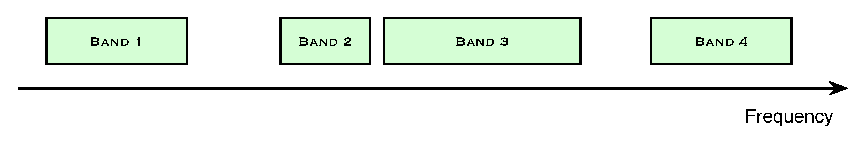
\includegraphics[width=.8\textwidth]{figures/Coord_FrequencyBands.eps}
  \end{center}
  The above figure shows gaps in the frequency axis for an observation
  with 4 bandpasses which are not similar in frequency range. This
  is typical for a LOFAR Beam-Formed type of observation \cite{lofar.icd.003}.
  
  A coordinate group to represent such a scenario would look like:
\begin{lstlisting}
.
`-- COORDINATES
    |- NOF_COORDINATES            2
    |- NOF_AXES                   2
    |- COORDINATE_TYPES           [`Time', `Spectral']
    |- COORDINATE_0
    |  |- COORDINATE_TYPE         `Time'
    |  |- STORAGE_TYPE            `Linear'
    |  |- NOF_AXES                1
    |  |- AXIS_NAMES              [`Time']
    |  |- AXIS_UNITS              [`s']
    |  |- REFERENCE_VALUE         [1.0]
    |  |- REFERENCE_PIXEL         [0.0]
    |  |- INCREMENT               [1.0]
    |  `- PC                      [1.0]
    `- COORDINATE_1
       |- COORDINATE_TYPE         `Spectral'
       |- STORAGE_TYPE            `Tabular'
       |- NOF_AXES                1
       |- AXIS_NAMES              [`Spectral']
       |- AXIS_UNITS              [`MHz']
       |- AXIS_LENGTH             1024
       |- AXIS_VALUES_PIXEL       [0, 1, 2, ..., 512, 513, ...]
       `- AXIS_VALUES_WORLD       [140, 140.1953125, 140.390625, ...,
                                   150, 150.1953125, ...]
\end{lstlisting}
\end{enumerate}

\section{Positions in space}

Following our data model, positions in space can be divided into two
basic groups:
\begin{enumerate}
\item Positions on spherical shells, using a spherical map projection
  onto a plane surface.
\item Positions in 3-dimensional space, as described through a set of
  cartesian, spherical, cylindrical, etc. coordinates.
\end{enumerate}

\subsection*{Position with spherical map projection}

\begin{comment}
  Mention in particular usage as part of the Sky Image. Extend the
  started examples to provide full set of attributes and values.
\end{comment}

\begin{enumerate}
\item Direction (angular position with spherical map projection) and
  radial component:
\begin{lstlisting}
.                                       .
|-- Direction [2]                          |-- Direction [2]
`-- Linear    [1]                          `-- Tabular   [1]
\end{lstlisting}
\item Direction (angular position with spherical map projection) with spectral
  component for Stokes $(I,Q,U,V)$ parameters.
\begin{lstlisting}
.
|-- Direction [2]
|-- Spectral  [1]
`-- Polarization    [1]
\end{lstlisting}
\end{enumerate}

\subsection*{Position without spherical map projection}

\begin{enumerate}
\item Cartesian coordinates, regular $(x,y,z)$ grid:
  \begin{enumerate}
  \item Single coordinate with three coordinates axes:
    \begin{lstlisting}
   COORDINATES
   `-- COORDINATE_0            Linear [3]
    \end{lstlisting}
  \item Three coordinates, each representing a single axis:
    \begin{lstlisting}
   COORDINATES
   |-- COORDINATE_0            Linear [1]
   |-- COORDINATE_1            Linear [1]
   `-- COORDINATE_2            Linear [1]
    \end{lstlisting}
  \end{enumerate}
\item Cartesian coordinates, regular $(x,y)$ grid, non-regular $z$-axis
  \begin{enumerate}
  \item Single coordinate for the two linear axes, tabular coordinate
    for the non-linear axis:
    \begin{lstlisting}
   COORDINATES
   |-- COORDINATE_0            Linear  [2]
   `-- COORDINATE_0            Tabular [1]
   \end{lstlisting}
  \item Three coordinates, each representing a single axis:
    \begin{lstlisting}
   COORDINATES
   |-- COORDINATE_0            Linear  [1]
   |-- COORDINATE_1            Linear  [1]
   `-- COORDINATE_2            Tabular [1]
    \end{lstlisting}
  \end{enumerate}
\item Cartesian coordinates, non-regular $x$-, $y$-, and $z$-axes
  \begin{lstlisting}
   COORDINATES
   |-- COORDINATE_0            Tabular [1]
   |-- COORDINATE_1            Tabular [1]
   `-- COORDINATE_2            Tabular [1]
  \end{lstlisting}
\end{enumerate}

%% _______________________________________________________________________________
%%                                                     Discussion & open questions

\chapter{Discussion}
\label{sec:discussion}

\section{Open questions/Issues}
\label{sec:open-questions}

The following table presents an overview of (some of the) known open
questions regarding the format definition:

\begin{center}
  \tablefirsthead{
    \hline
    \sc Item & \sc Description & \sc Status \\
    \hline
  }
  \tablehead{
   \multicolumn{3}{r}{\small\sl continued from previous page} \\
    \hline
    \sc Item & \sc Description & \sc Status \\
    \hline
  }
  \tabletail{
    \hline
    \multicolumn{3}{r}{\small\sl continued on next page} \\
 }
 \tablelasttail{\hline}
 \begin{supertabular}{lp{12.8cm}l}
   01 &  Compare guidelines on physical units from IAU Style Manual
   \cite{mcnally.1988} with guidelines/definitions in ESO ICDs and IOVA manuals
   (e.g. \cite{ivoa.stc}). & open \\
   02 & Copy Table 1 of \cite{fits.paper3} to ICD. & open \\
   03 & Motivation for reference frame keywords in both spectral coordinate and
   coordinates group: ``The parameters needed to compute geocentric
   frequencies/velocities from topocentric are the siderial time and the observation
   location. The observation date is needed to convert from geocentric to barycentric
   coordinates.'' \cite{fits.paper3} & open \\
   04 & Provide translation scheme onto representation in FITS \cite{fits.paper1,fits.paper2,fits.paper3}. & open \\
   05 & Add figures with position grids of spatial coordinates & open
   \\
   06 & What exactly is the difference between the separate conventions (e.g
   see \cite{straten.2009})? Is this something simple like e.g. a
   different sign in front of the $\omega t$? Work out who this
   actually affects the standard Stokes parameters. & open \\
 \end{supertabular}
\end{center}

\section{Future enhancements}
\label{sec:future-enhancements}

---/---

%% ______________________________________________________________________________
%%                                                                     References

\clearpage

\bibliographystyle{abbrv}     %% abbrv | plain
\bibliography{references}

\chapter*{\glossaryname}
\label{sec:glossary}
\addcontentsline{toc}{section}{\glossaryname}

\input lofar_common_glossary

%% ==============================================================================
%%
%%  Appendices
%%
%% ==============================================================================

% \clearpage
% \appendix

\end{document}


%% ==============================================================================
%%
%%  Additional material not included in the document 
%%
%% ==============================================================================

\chapter*{Parametrization of polarization properties.}

The \textsl{coherence matrix} is defined by \cite{bladel.2007}
\begin{eqnarray}
  \label{eq:1}
  \overline{\overline \Gamma} & = & \left(
    \begin{array}{cc}
      \langle E_x E_x^\ast \rangle & \langle E_x E_y^\ast \rangle \\
      \langle E_y E_x^\ast \rangle & \langle E_y E_y^\ast \rangle
    \end{array}
  \right)
\end{eqnarray}
This matrix is Hermitian. The diagonal elements are positive; hence,
the trace of the matrix is positive as well. Normalization to unit
trace yields the \textsl{polarization matrix} $\overline{\overline
  p}$. For example:
\begin{itemize}
\item In a time-harmonic linearly polarized field making an angle
  $\gamma$ with the $x$-axis, $\overline\overline p$ is given by
  \begin{eqnarray}
    \label{eq:3}
    \overline\overline p & = & \left(
      \begin{array}cc}
        \cos^2 \gamma & \sin \gamma \cos \gamma \\
        \sin \gamma \cos \gamma & \sin^2 \gamma
      \end{array}
    \right)
  \end{eqnarray}
\item In a time-harmonic circularly polarized field,
  \begin{eqnarray}
    \label{eq:5}
    \overline\overline p & = & \left(
      \begin{array}{cc}
        0.5 & \pm 0.5 i \\
        \mp 0.5 i & 0.5
      \end{array}
    \right)
  \end{eqnarray}
  
\end{itemize}

Both intensity and state of polarization can be efficiently
characterized by the -- real -- \textsl{Stokes parameters}
\begin{equation}
  \begin{array}{lllllll}
    s_0 & = & I & = & \langle E_x E_x^\ast \rangle + \langle E_y
    E_y^\ast \rangle & = & \Gamma_{xx} + \Gamma_{yy} \\
    s_1 & = & Q & = & \langle E_x E_x^\ast \rangle - \langle E_y
    E_y^\ast \rangle & = & \Gamma_{xx} - \Gamma_{yy} \\
    s_2 & = & U & = & 2 {\rm Re} \langle E_x E_y^\ast \rangle & = &
    \Gamma_{xy} + \Gamma_{yx} \\
    s_3 & = & V & = & - 2 {\rm Im} \langle E_x E_y^\ast \rangle & = &
    i \left( \Gamma_{xy} - \Gamma_{yx} \right)
  \end{array}
\end{equation}

